\documentclass[11pt]{article}
\usepackage{graphicx} % Required for inserting images
\usepackage{indentfirst}
\usepackage[a4paper, margin=3cm]{geometry}
\usepackage[main=ngerman]{babel}
\usepackage{hyperref}

\setlength{\parskip}{5pt}
\graphicspath{./images/}
\hypersetup{linktoc=all}

\title{VL1-Einführun}
\author{Metin Eren Heybet}
\date{14 Oktober 2024}

\begin{document}

\maketitle

\tableofcontents
\newpage

\section{Einführung - allgemeine Informationen}

\subsection{steigender Leitungsbedarf}

\begin{itemize}
    \item Heutzutage erfordern größere Probleme immer schnellere Systeme, z.B Klimasimulationen, animierte Filme usw.
    \item Mit mehr Rechenleistung steigt der Appetit auf anspruchvollere Anwendungen, wobei auch Energieeffizienz wichtig ist.
    \item Leitungsanforderungen im Tera-/Petaflopsbereich \footnote{FLOP = Floating Point Operations}
\end{itemize}

\subsection{Moore's Law und die Entwicklung der verschiedenen Aspekten von Hardware}

\begin{itemize}
    \item Die Prozessorgeschwindigkeit verdoppelte sich bis ca. 2005 alle 18 Monate.
    \item \textbf{Memory Wall:} Währenddessen die Hauptspeicherzugriffgeschwindigkeit sich nur etwas alle 10 Jahre verdoppelt hat.
    \item \textbf{Frequency Wall:} Erhöhung der Taktfrequenzen und längere Pipelines erzielen keine höhere Rechenleistung mehr.
    \item Deswegen steigt heutzutage die Bedeutung von Multi-Core-Architekturen
\end{itemize}

\section{Multi-Core-Architekturen}
Multicore-Architekturen sind allgegenwärtig sowohl im High-Performance-Computing als auch im Heimanwenderbereich.

Sie stellen eine mögliche Lösung für die Probleme der Hardware-Entwicklung dar.

Leider passiert diese kürzere Laufzeiten nicht automatisch: Man muss für mehr CPUs \textbf{parallel programmieren}.

\subsection{Vorteile von Parallelität in Programme}
\begin{itemize}
    \item Reduktion der Bearbeitungszeit für ein Problem
    \item Höherer Durchsatz der Anwendungsprogramme
    \item Höhere Reaktionsgeschwindigkeit
    \item Klarere Programmstrukturen, insbesondere für Aktivitäten, die externe Geräte steuern.
\end{itemize}

\subsection{Die Vorteile von Funktionale Programmierung}
\begin{itemize}
    \item Datenabhängigkeiten in dem Code erschweren die fehlerfreie Programmierung, sowohl von sequentiellem als auch parallelem Code.
    \item Mit funktionalen Sprachen kann man diese Komplexität für den Programmierer reduzieren.
\end{itemize}

\section{Arte von Prozessen}
%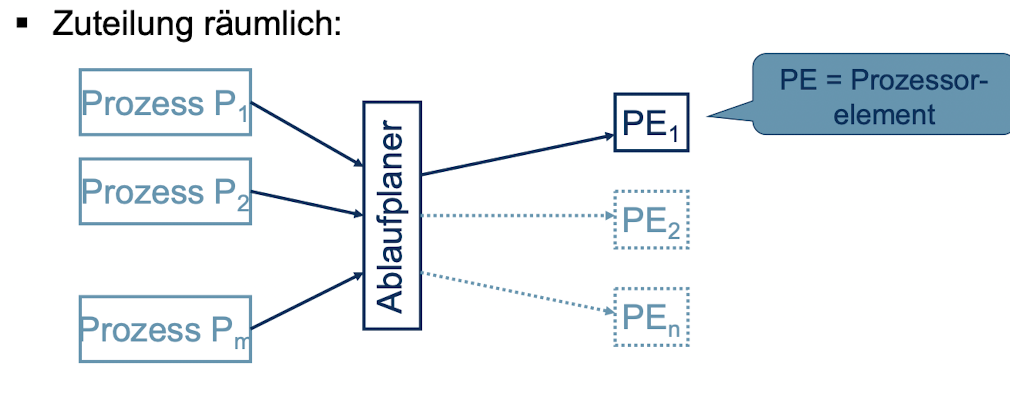
\includegraphics[width=0.9\linewidth]{images/photo1}
\end{document}
